\documentclass[aps,twocolumn,showpacs]{revtex4-1}


\usepackage{epsfig}
\usepackage{amsfonts}
\usepackage{amssymb}
\usepackage{mathrsfs}
\usepackage{theorem}
\usepackage{amsmath}
\usepackage{times}
\usepackage{color}
\usepackage[french]{babel}
\usepackage[T1]{fontenc}
\usepackage{ifpdf}
\ifpdf
\usepackage{epstopdf}   
\usepackage{url}
\fi


\begin{document}
\title{Probing dark spins with NV centers in CVD-grown diamond}

\author{Clément Pellet-Mary$^{1}$, Maxime Perdriat$^1$, Paul Huillery$^1$, Alexandre Tallaire$^2$ and Gabriel Hétet$^1$}
%\email{gabriel.hetet@phys.ens.fr}
\affiliation{$^1$Laboratoire De Physique de l'\'Ecole Normale Sup\'erieure, 24 rue Lhomond, 75231 Paris Cedex 05, France. \\
$^2$ IRCP, Ecole Nationale Sup\'erieure de Chimie de Paris, 11 rue Pierre et Marie Curie, 75005 Paris, France
}

\begin{abstract}
\normalsize
The electronic spin of the Nitrogen Vacancy (NV) center in diamond has given rise to a wealth of application over the past ten years, in particular in the domain of magnetic field sensing. The main reason to its rapid rise in popularity is the ability of the spin to be optically polarized and read-out at room temperature, with nothing more than a confocal microscopy setup. 

Because of their point-like nature, NV centers can be placed a few nanometers away from the magnetic source, making them good candidate to probe tiny fields, such as the ones produced by other spins. Electronic and nuclear spins, both inside or outside the diamond have been detected by NV center magnetometry, down to a single spin \citep{Ref1}.

In our work \citep{Ref2}, we have used a diamond grown through chemical vapor deposition (CVD) with a relatively large ensemble of NV centers ($\approx$~3 ppm) in order to probe trace amounts of other electronic spins in the diamond, in the ppb range. This technique relies on resonant dipole-dipole coupling between the spins (flip-flop) \citep{Ref3} and unlike many NV magnetometry protocols does not require a microwave field. 

Compared to traditional electronic spin resonance technique such as EPR, besides its comparatively simpler apparatus and potential gain in sensibility, an NV-based method present the advantage not to rely on the total number of spins of the sample, but rather only on the spins in the vicinity of the probed NV centers, making the measurement applicable to micro or nano-diamond, with a spatial resolution given by the diffraction limit of the microscope.

Understanding and controlling the local environment of NV-centers is a key aspect to improve NV magnetometry and other quantum applications with NV centers. Our method could provide chemists and material scientists a quick and cheap purity test for the samples they grow.
\begin{figure}[h]
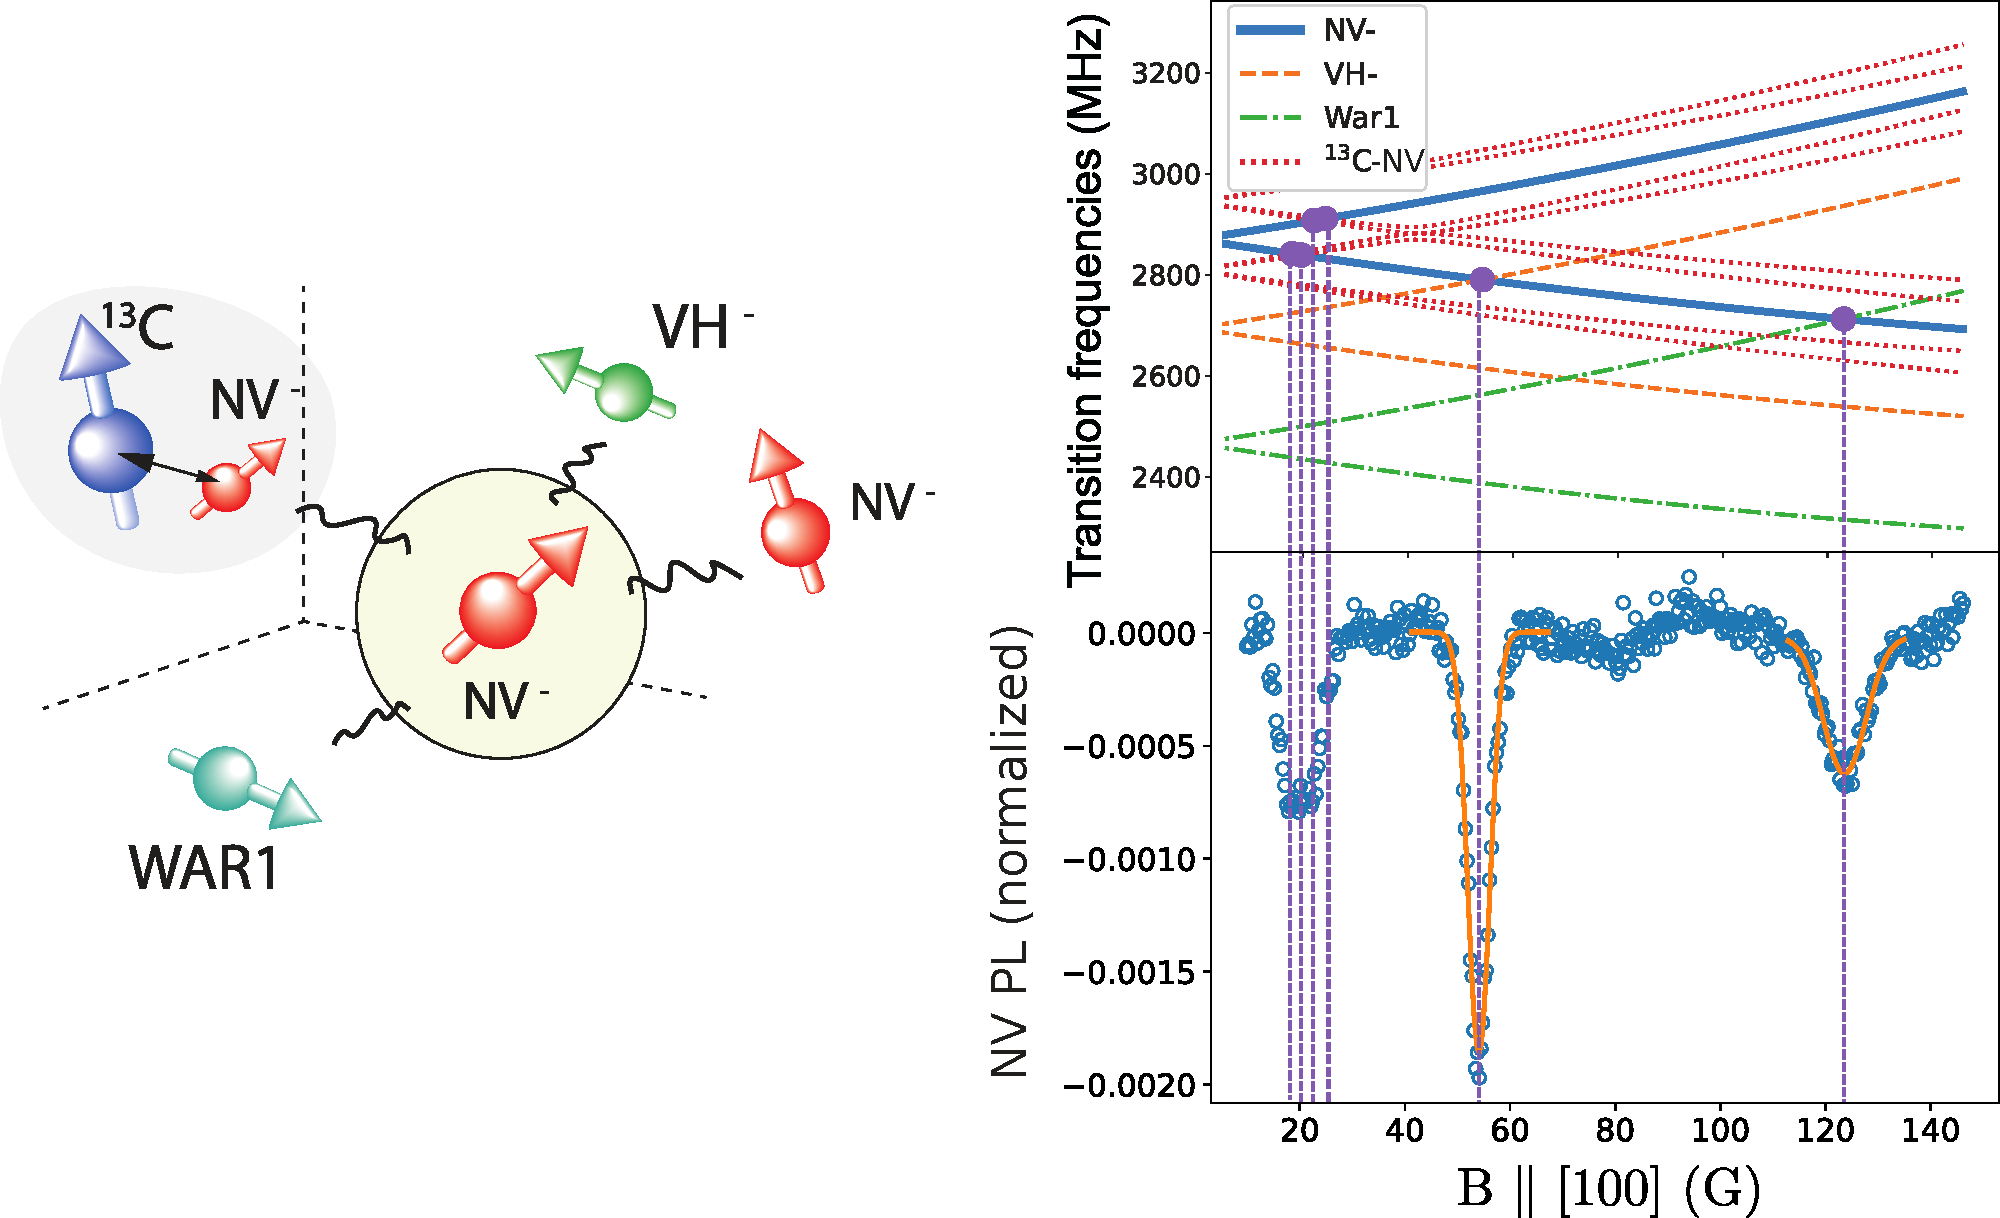
\includegraphics[scale=0.3]{Fig}
\caption{\textbf{Top Figure :} Transition energies of the NV center's spin and various dark spins as a function of the external magnetic field.\\ \textbf{Bottom figure : }Normalized photoluminescence of the NV center as a function of the external magnetic field. \\Resonant dipolar coupling between polarized NV centers and unpolarized dark spins induce a depolarization of the NV spin which is detected by a drop in the NV photoluminescence}
\end{figure}
\end{abstract}

\maketitle

\begin{thebibliography}{}

\bibitem{Ref1} Zhao, Nan, et al. Nature nanotechnology 7.10 (2012): 657-662.

\bibitem{Ref2} Pellet-Mary, C., Huillery, P., Perdriat, M., Tallaire, A., Hétet, G. (2021). Physical Review B, 103(10), L100411.

\bibitem{Ref3} Armstrong, S., Rogers, L. J., McMurtrie, R. L., Manson, N. B. (2010). Physics Procedia, 3(4), 1569-1575.
\end{thebibliography}
\end{document}
